\section{Components}
\label{sec:components}
Just like in Unity, the components are the building blocks of the game objects.
They are the individual features that can be added to a game object to give it functionality.

\subsection{class diagram}
\begin{figure}[H]
    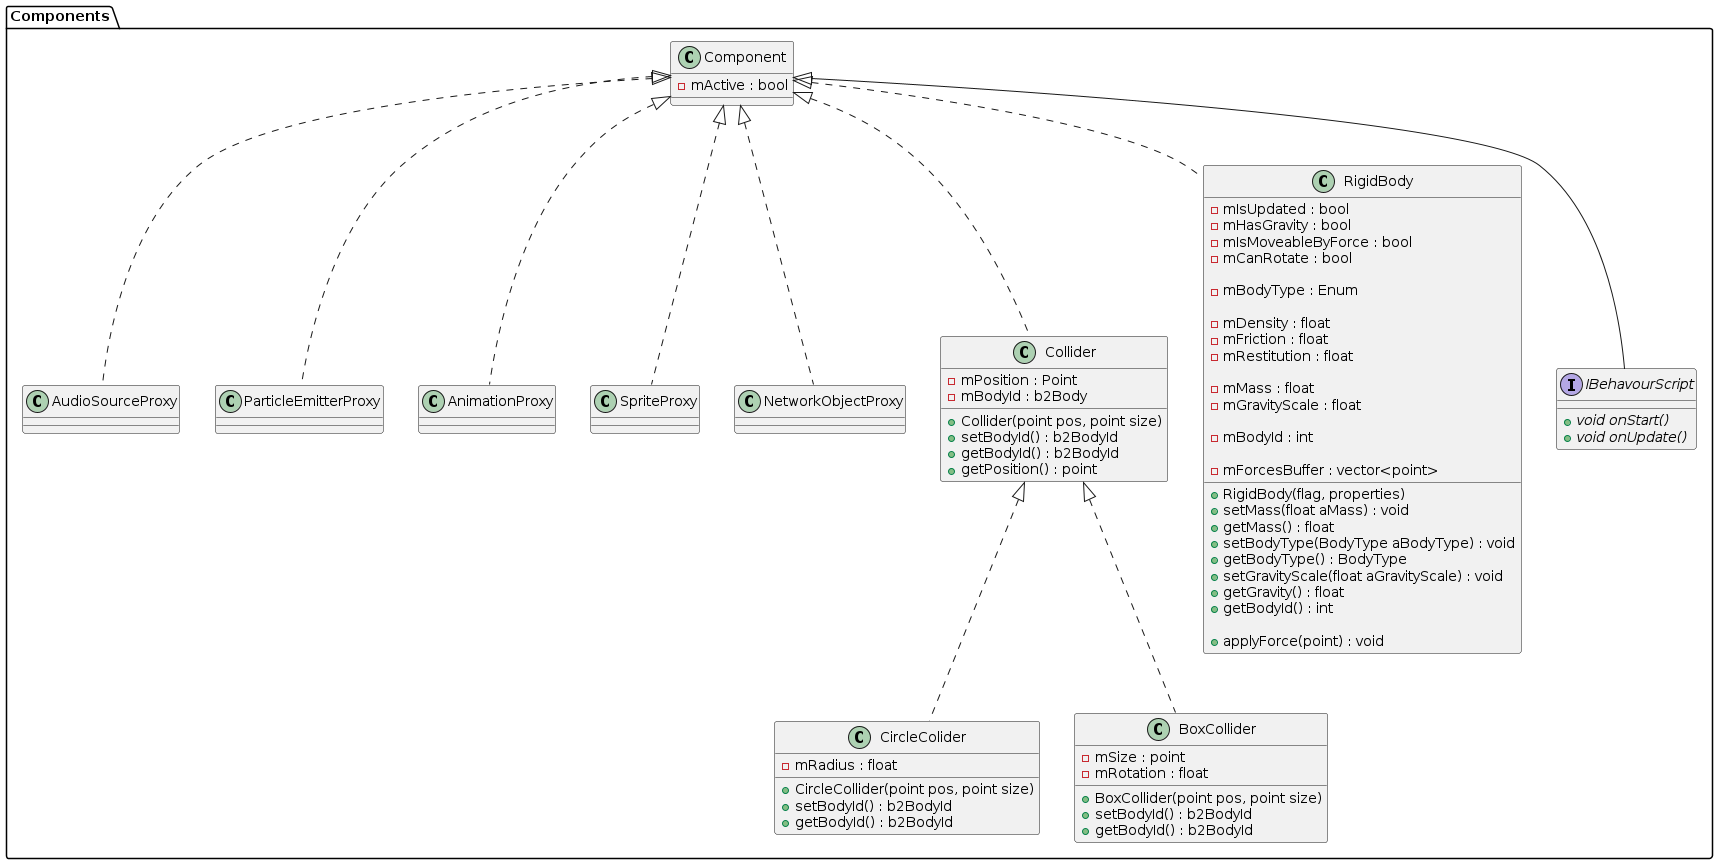
\includegraphics[width=1.2\textwidth]{componentsPackageClassDiagram.png}
    \caption{Class diagram of the components}
    \label{fig:components}
\end{figure}

\subsection{Collider}
Has \texttt{bodyID}, which is needed for the physics.

\subsection{NetworkObject}

\subsection{Sprite}

\subsection{Animation}

\subsection{IBehaviourScript}

\subsection{RigidBody}
Has \texttt{bodyID}, which is needed for the physics.

\subsection{Sprite}
Used to add a texture to a GameObject.

\subsection{IBehaviourScript}
IBehaviour script is an interface that can be used to create behaviour scripts for GameObjects.

\subsection{ParticleEmitter}
Used to create particle effects.

\subsection{AudioSource}
Used to add audio to a GameObject.
\subsection{Transform}

Does not need an update flag when the position is changed, as a movable object is usually moving.


